\documentclass{beamer}

\mode<presentation> {

\usetheme{Boadilla}

}
\setbeameroption{show notes}
\usepackage{multirow}

\usepackage{algorithmic}
\usepackage{algorithm}
\usepackage{booktabs}
\usepackage{listings}
\usepackage{xcolor}
\newcommand\myworries[1]{\textcolor{red}{#1}}
\usepackage{hyperref} 
\usepackage{natbib}
\usepackage{subfig}
\usepackage{color}
\usepackage{placeins}
\usepackage[utf8]{inputenc}
\usepackage{graphicx} % Allows including images
\usepackage{booktabs} % Allows the use of \toprule, \midrule and \bottomrule in tables


%\setbeameroption{show notes}
%----------------------------------------------------------------------------------------
%	TITLE PAGE
%----------------------------------------------------------------------------------------


\title[Seminar]{Medujezično prepoznavanje imenovanih entiteta pomoću wikifikacije} % The short title appears at the bottom of every slide, the full title is only on the title page

\author{Stipan Mikulić} % Your name
\institute[FER]{
\textit{Mentor: doc. dr. sc. Jan Šnajder}\\
\medskip
Fakultet elektortehnike i računarstva \\
Sveučilište u Zagrebu \\
}
\date{1. lipnja 2017.}

\begin{document}



\begin{frame}
\titlepage % Print the title page as the first slide
\end{frame}

\note[]{
Dobar dan svima. Ja sam Stipan Mikulić. Tema moga seminara je medujezicko prepoznavanje imenovanih entiteta pomocu wikifikacije.
}

\begin{frame}
\frametitle{Sadržaj} % Table of contents slide, comment this block out to remove it
\tableofcontents
\end{frame}

\note[]{
}



%----------------------------------------------------------------------------------------
%	PRESENTATION SLIDES
%----------------------------------------------------------------------------------------


\section{Opis problema i motivacija}
\begin{frame}
\frametitle{Opis problema i motivacija}
\begin{itemize}
\item za razvoj dobrog modela potrebno je puno podataka
\item više od 50\% sadržaja na internetu je na engleskom jeziku
\item Referencirani rad: Chen-Tse Tsai and Stephen D. Mayhew and Dan Roth, Cross-Lingual Named Entity Recognition via Wikification,
\end{itemize}
\end{frame}

\note[]{
Za razvoj dobrog modela za klasifikaciju potrebno nam je puno podataka. 

Prema zadnjim procjenama više od 50\% sadžaja na internetu je pisano na engleskom jeziku. U potpunoj dominaciji engleskog jezika u svim vrstama podataka i NLP alata i leži motivacija za razvoj medjezičnog modela.
}
\begin{frame}
\frametitle{Opis problema i motivacija}
Prepoznavanje imenovanih entiteta je zadatak klasifikacije elemenata u predefinirane kategorije kao što su:

\begin{itemize}
	\item Imena -- Osobe, Organizacije, Lokacije
	\item Vremenske oznake -- Vrijeme, Datum
	\item Brojevi -- Novac, Postotci
	\item ...
\end{itemize}

[Jim]\textsubscript{OSOBA} bought [300]\textsubscript{BROJ} shares of [Acme Corp.]\textsubscript{ORGANIZACIJA} in [2006]\textsubscript{VRIJEME}.

\end{frame}
\note[]{

Prepoznavanje imenovanih entiteta je zadatak ekstrakcije informacija kojem je cilj klasificirati u predefinirane kategorije kao što su:
• Imena – Osobe, Organizacije, Lokacije
• Vremena – Vrijeme, Datum
• Brojevi – Novac, Postotci

Ovisno o domeni za koju se koriste imenovani entiteti, moguće ih je prizvoljno definirati. 

U ovom primjeru entitet OSOBA sadrži jedan token dok entitet ORGANIZACIJA sadrži dva tokena.
}

\begin{frame}
\frametitle{Opis problema i motivacija}
Kategorije eniteta u ovom radu:

\begin{itemize}
	\item PER -- Osobe
	\item ORG -- Organizacije
	\item LOC -- Lokacije
	\item MISC -- Razno
\end{itemize}
\end{frame}


\section{Analiza podataka}
\begin{frame}
\frametitle{Analiza podataka}

\begin{itemize}
\item CoNLL -- Conference on Computational Natural Language Learning
\item izvor podataka: CoNLL02 i CoNLL03 
\item španjolski i nizozemski označeni u BIO format.
\item engleski prebačen iz IO u BIO format.
\end{itemize}
\end{frame}
\note[]{
Format u kojem se s B označavaju riječi na početku entiteta, I označavaju riječi unutar entiteta i O označavaju riječi koje ne pripadaju ni jednom entitetu. 

Format u kojem se s označavaju riječi koje pripadaju nekom entitetu i O označavaju riječi koje ne pripadaju ni jednom entitetu.
}




\begin{frame}
\frametitle{Broj entiteta u skupovima}
\begin{center}
\begin{tabular}{ clcccc }
\hline
\textbf{jezik} & \textbf{skup} & \textbf{PER} & \textbf{ORG} & \textbf{LOC} & \textbf{MISC} \\ \hline
\multirow{3}{*}{eng} & train & 6600 & 6321 & 7140 & 3438 \\
 & validation & 1842 & 1341 & 1837 & 922 \\
 & test & 1617 & 1661 & 1668 & 702 \\ \hline
\multirow{3}{*}{esp} & train & 4321 & 7390 & 4913 & 2173 \\
 & validation & 1222 & 1700 & 984 & 445\\
 & test & 735 & 1400 & 1084  & 339 \\ \hline
\multirow{3}{*}{ned} & train & 4716 & 2082 & 3208 & 3338 \\
 & validation & 703 & 686 & 479 & 748 \\
 & test & 1098 & 882 & 774 & 1187 \\ \hline
\end{tabular}
\end{center}\end{frame}


\begin{frame}
\frametitle{Veličina entiteta skupa podataka na engleskom jeziku}
\begin{center}
  \makebox[\textwidth]{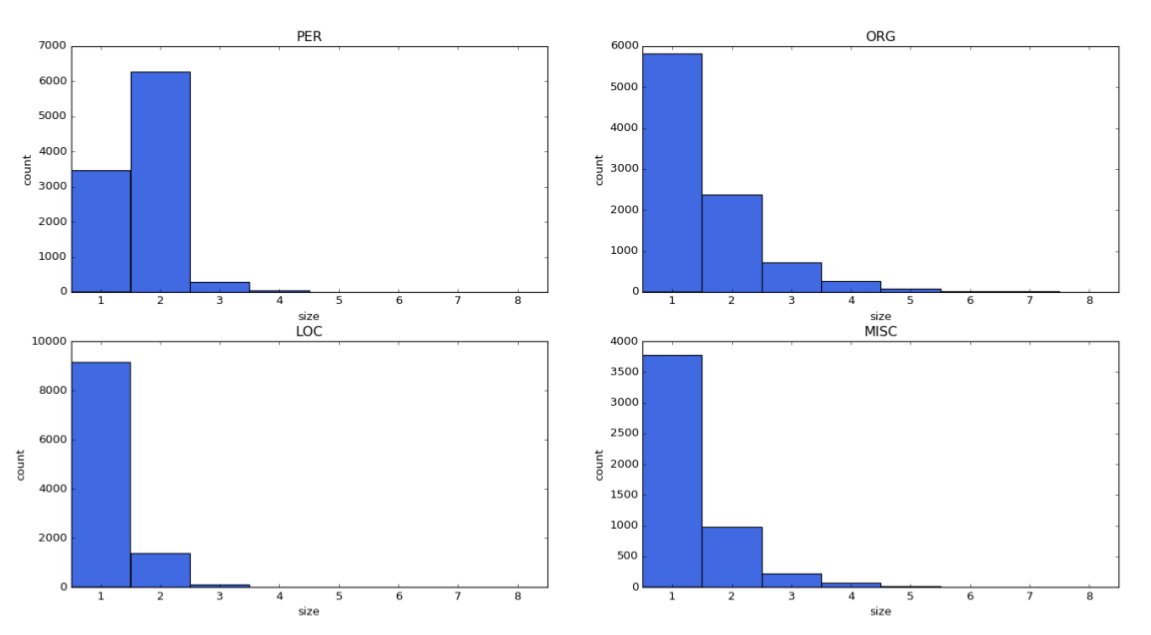
\includegraphics[scale=0.2]{images/engpod.png}}
\end{center}
\end{frame}

\begin{frame}
\frametitle{Veličina entiteta skupa podataka na španjolskom jeziku}
\begin{center}
  \makebox[\textwidth]{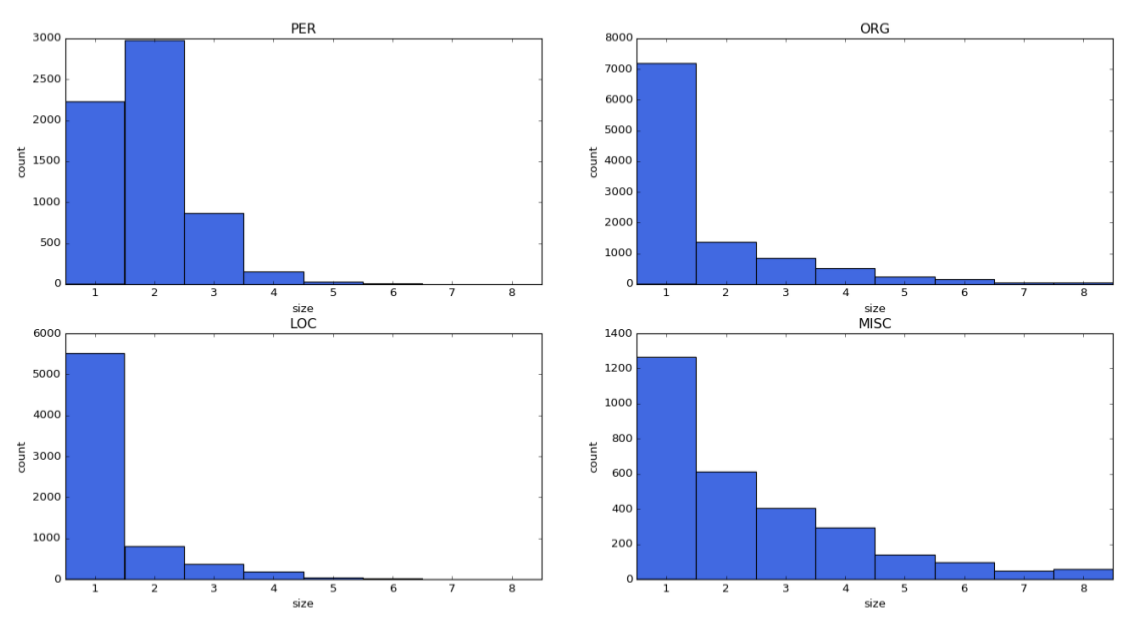
\includegraphics[scale=0.2]{images/esppod.png}}
\end{center}
\end{frame}

\begin{frame}
\frametitle{Veličina entiteta skupa podataka na nizozemskom jeziku}
\begin{center}
  \makebox[\textwidth]{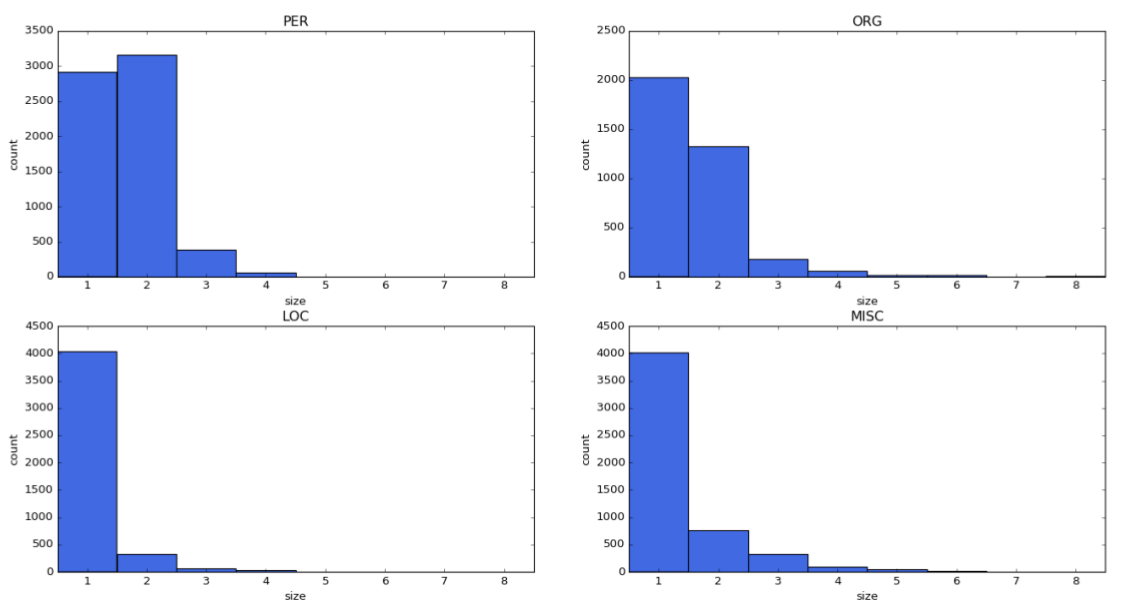
\includegraphics[scale=0.2]{images/nedpod.png}}
\end{center}
\end{frame}


\section{Modeli}
\begin{frame}
\frametitle{Modeli}
\begin{itemize}
\item Modeli iz scikit-learn knjižnice:
\item Perceptron
\item Logistička regresija
\item modeli trenirani na 200 iteracija
\item balansirane klase pri treniranju
\end{itemize}
\end{frame}
\note[]{
parametar je postavljen na "balanced" što znači da model klase koje se rijetko pojavljuju unutar skupa za treniranje kažnjava više za grešku u predikciji jer sve klase smatra jednakima. Modeli su trenirani na 200 iteracija.
}

\section{Značajke}
\begin{frame}
\frametitle{Skupovi značajki}
\begin{enumerate}
\item Osnovni model (engl. baseline) 
\item Osnovni model + Gazeteri
\item Osnovni model + Gazeteri + Wikifikacija
\end{enumerate}
\begin{center}
\captionof{table}{Broj gazetera za svaki entitet}
\begin{tabular}{ lcccc }
\hline
 & PER & LOC & ORG & MISC\\ 
\hline
Gazeteri & 2 972 k & 3 106 k & 977 k & 2 991 k \\
\hline
\end{tabular}
\end{center}
\end{frame}
\note[]{

\textbf{Gazeteri} su unaprijed prikupljeni skupovi entiteta. 
\textbf{Wikifikacija} je proces prepoznavanja entiteta u tekstu te povezivanja istih s nasličnijim stranicama na wikipediji.

}

\begin{frame}
\frametitle{Engleska wikifikacija}
\begin{center}
  \makebox[\textwidth]{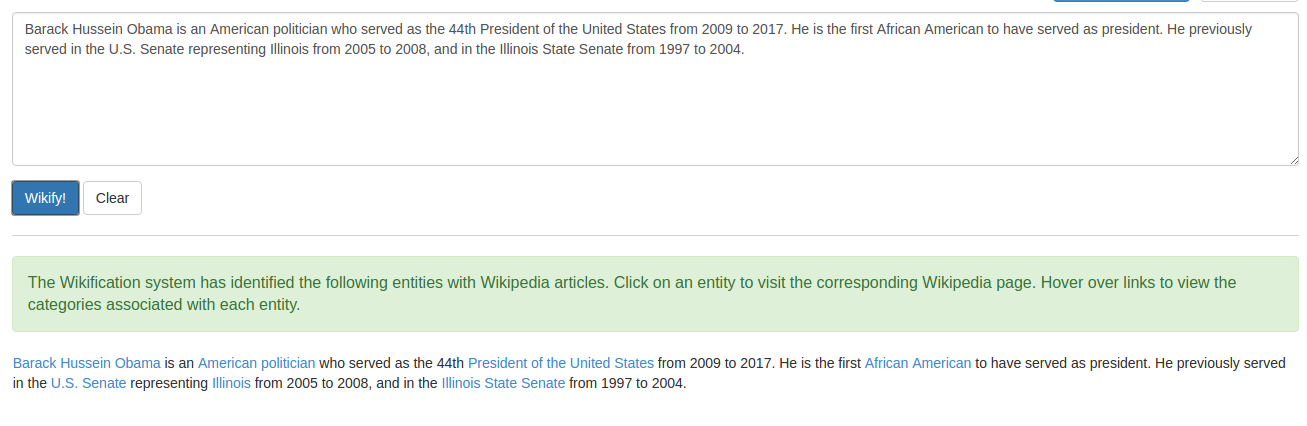
\includegraphics[scale=0.25]{images/eng.png}}
\end{center}
\end{frame}


\begin{frame}
\frametitle{Španjolska wikifikacija}
\begin{center}
  \makebox[\textwidth]{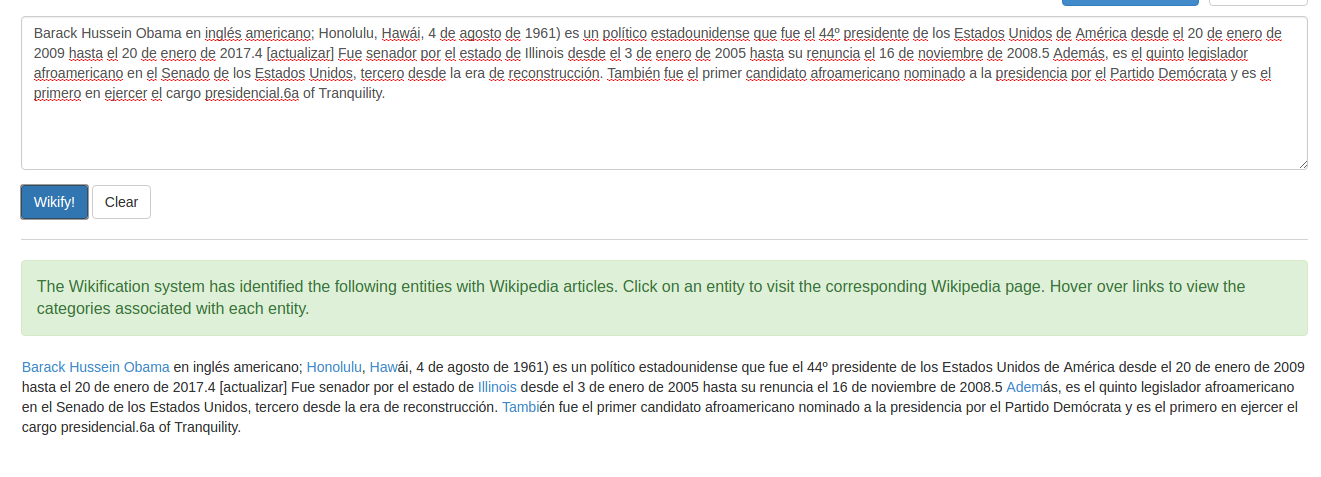
\includegraphics[scale=0.25]{images/esp.png}}
\end{center}
\end{frame}


\begin{frame}
\frametitle{Nizozemska wikifikacija}
\begin{center}
  \makebox[\textwidth]{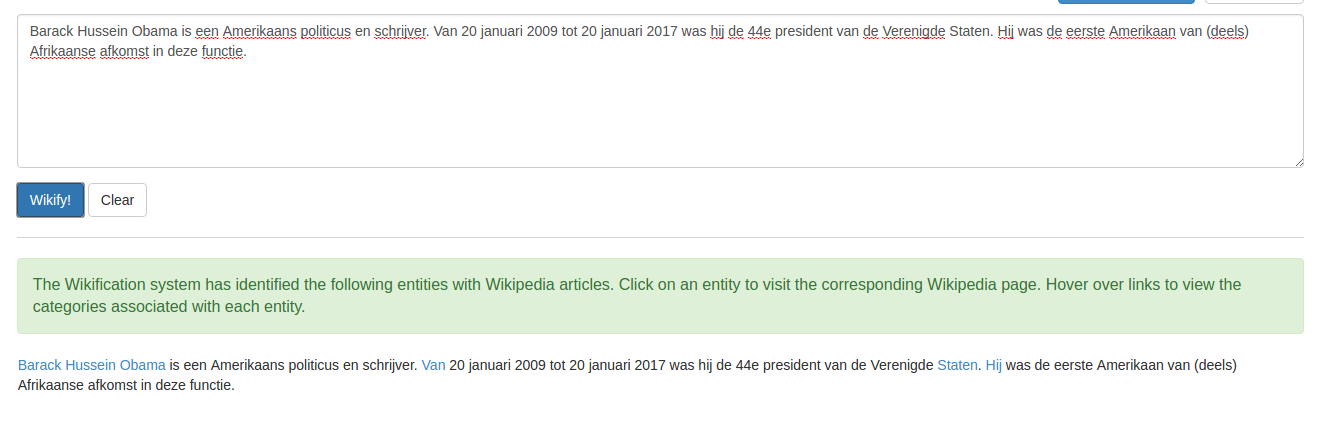
\includegraphics[scale=0.25]{images/ned.png}}
\end{center}
\end{frame}


\begin{frame}
\frametitle{Značajke}
\begin{center}
\begin{tabular}{llr}
\hline
\textbf{Osnovne značajke} & \\
prethodni tag entiteta & $ (t_{i-1},t_{i-2}) $\\ 
sadrži samo brojke i slova & $ alphanumeric(w_i) $\\ 
sadrži samo brojke  & $ alldigits(w_i) $\\ 
sadrži samo velika slova & $ allcaps(w_i) $\\ 
sadrži samo brojke & $ iscap(w_{i-2}, w_{i-1}, w_{i}, w_{i+1}, w_{i+2}) $\\
3-gram & suma pojavljivanja za svaku klasu \\
\textbf{Gazeteri} & \\
naziv kategorije gazetera  & $ topic(w_{i}, w_{i+1}, w_{i+2}, w_{i+3}) $\\
broj pojavljivanja riječi u kategoriji & $ cat\_count(w_{i}, \{PER, LOC, ORG\}) $\\
\textbf{Medujezične značajke} & \\
--- & ---\\

\hline
\end{tabular}
\end{center}
\end{frame}
\note[]{
Za potrebe ovog modela prikupljeni gazeteri su podijeljeni u teme čiji su naslovi korišteni kao značajke modela. Neke od tema su: ArtWork, Building, Clothes, Films, Parks, Vehicles itd. Dodatno su prikupljeni skupovi za entitete Osoba, Organizacija i Lokacija te su za značajke korišteni kao broj pojavljivanja riječi u pojedinom skupu.

}

\begin{frame}
\frametitle{Pretprocesiranje značajki}
\begin{itemize}
\item kategoričke značajke -- Onehot coding
\item brojčane značajke -- MinMaxScaler(0, 1)
\end{itemize}
\end{frame}
\note[]{

Većina korištenih značajki su kategoričke stoga su kodirane Onehot metodom. 

Brojčane značajke kojima je definiran poredak skalirane su na interval $ [0,1] $. Za skaliranje je korišten MinMaxScaler

}

\begin{frame}
\frametitle{Unakrsna validacija}
Parametri perceptrona: 
\[ alpha = (10^{-10}, 10^{-9}, ..., 10^{-2}) \]
\[ penalty = (l2, l1) \]

Parametri logističke regresije:

\[ c = (10^{-7}, 10^{-9}, ..., 10^{2}) \]
\[ penalty = (l2, l1) \]
\end{frame}

\section{Evaluacija}
\begin{frame}
\frametitle{Evaluacija}
Sustav je evaluiran na dva način:
\begin{enumerate}
\item Standardne mjere na razini svakog tokena.
\item Točno podudaranje gdje se entitet smatra dobro predvidenim ako se svaki token podudara po tipu s označenim podatcima.

\begin{center}
\captionof{table}{Veličina skupova podataka}
\begin{tabular}{ lccc }
\hline
 & ENG & ESP & NED \\ 
\hline
Entiteti (treniranje) & 29 441 & 23 148 & 15 960 \\
Entiteti (testiranje) & 5 648 & 3 558 & 3 941 \\
\hline
\end{tabular}
\end{center}
\end{enumerate}
\end{frame}
\note[]{

}

\begin{frame}
\frametitle{Standardne evaluacijske mjere}
\begin{center}
\scalebox{0.9}{
\begin{tabular}{ lcccc|cccc }
\hline
& \multicolumn{4}{c}{Perceptron} & \multicolumn{4}{c}{Log. regresija} \\ 
\cline{2-5}\cline{6-9}
 & ENG & ESP & NED & AVG & ENG & ESP & NED & AVG\\ 
\hline
\multicolumn{9}{c}{Jednojezični eksperimenti } \\
\hline
Osnovne značajke & 0.66 & 0.64 & 0.55 & 0.62 & 0.62 & 0.62 & 0.59 & 0.61 \\
+Gazeteri & 0.67 & 0.64 & 0.58 & 0.63 & 0.70 & 0.64 & 0.68 & 0.67 \\
+Wikifikacija & -- & -- & -- & -- & -- & -- & -- & -- \\
\hline
\multicolumn{9}{c}{Medujezični eksperimenti } \\
\hline
Osnovne značajke & -- & 0.59 & 0.56 & 0.575 & -- & 0.63 & 0.66 & 0.645 \\
+Gazeteri & -- & 0.61 & 0.54 & 0.575 & -- & 0.64 & 0.63 & 0.635\\
+Wikifikacija & -- & -- & -- & -- & -- & -- & -- & -- \\
\hline
\end{tabular}}
\end{center}
\end{frame}

\begin{frame}
\frametitle{Evaluacija metodom točnog podudaranja}

\begin{center}
\scalebox{0.9}{
\begin{tabular}{ lcccc|cccc }
\hline
& \multicolumn{4}{c}{Perceptron} & \multicolumn{4}{c}{Log. regresija} \\ 
\cline{2-5}\cline{6-9}
 & ENG & ESP & NED & AVG & ENG & ESP & NED & AVG\\ 
\hline
\multicolumn{9}{c}{Jednojezični eksperimenti } \\
\hline
Osnovne značajke & 0.46 & 0.43 & 0.38 & 0.42 & 0.73 & 0.75 & 0.67 & 0.72 \\
+Gazeteri & 0.51 & 0.44 & 0.43 & 0.46 & 0.78 & 0.77 & 0.72 & 0.76 \\
+Wikifikacija & -- & -- & -- & -- & -- & -- & -- & --  \\
\hline
\multicolumn{9}{c}{Medujezični eksperimenti } \\
\hline
Osnovne značajke & -- & 0.29 & 0.31 & 0.30 & -- & 0.46 & 0.47 & 0.465 \\
+Gazeteri & -- & 0.33 & 0.28 & 0.305 & -- & 0.44 & 0.41 & 0.425 \\
+Wikifikacija & -- & -- & -- & -- & -- & -- & -- & --  \\
\hline
\end{tabular}}
\end{center}
\end{frame}


\begin{frame}
\begin{center}
  \makebox[\textwidth]{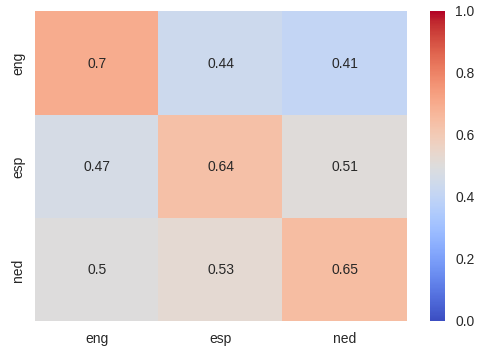
\includegraphics[scale=0.5]{images/corr_plot.png}}
\captionof{figure}{Evaluacijska matrica modela s različitim jezicima za treniranje i testiranje. Korištena je f1 mjera. Evaluacija je izvršena na modela koji uključuje baseline i gazetere.}
\end{center}
\end{frame}

\begin{frame}

\begin{center}
\frametitle{Poboljšanja}
\begin{itemize}
\item bolji odabir tema za gazetere
\item dodavanje novih značajki
\item podešavanje wikifiera
\end{itemize}
\end{center}
\end{frame}
\note[]{
Poboljšanja se kriju u boljoj kvaliteti podataka i otkrivanju nekih bolji značajki. Konkretno za razvijeni model u ovom radu pri odluci koji tema gazettera će biti dodjeljena
trenutno promatranoj riječi dobije se pronalaskom te riječi u skupu teme. 
Poboljšanje možemo ostvariti presjekom tema s okolnim riječima jer ne pripada neka riječ samo
jednoj temi. 
Uključivanje word embeddinga kao značajke za svaku riječ bi moglo re-
zultirati poboljšanjem. Metoda Wikifikacije se može poboljšati boljom distribucijom
kategorija i obogaćivanjem wikipedije za jezike s manjim resursima.
}

\begin{frame}
\begin{center}
\Huge Hvala na pažnji! \\
 Pitanja?
\end{center}

\end{frame}

\end{document} 